\documentclass[12pt]{article}
\usepackage[english]{babel}
\usepackage[utf8]{inputenc} % Permite el uso de caracteres del Español
\usepackage[T1]{fontenc}
\usepackage{graphicx}
\usepackage{amsmath}
\usepackage{wrapfig}
\usepackage{enumerate}
\usepackage[top=1in, bottom=1.25in, left=1.1in, right=1.1in]{geometry}
\usepackage[dvipsnames]{xcolor}
\usepackage{subcaption}

\begin{document}

\begin{titlepage}

\newcommand{\HRule}{\rule{\linewidth}{0.5mm}} % Define un comando para las lineas horizontales

\center 
%----------------------------------------------------------------------------------------
%	Cabezera
%----------------------------------------------------------------------------------------

\textsc{\LARGE Universidad de Sonora}\\[1.5cm]
\textsc{\Large Licenciatura en Física}\\[0.5cm]
\textsc{\large Física Computacional I}\\[0.5cm]

%----------------------------------------------------------------------------------------
%	Titulo
%----------------------------------------------------------------------------------------

\HRule \\[0.4cm]
{\huge \bfseries Actividad 5 - Preparando datos con ayuda de Emacs}\\[0.4cm] % Title of your document
\HRule \\[1.5cm]
 
%----------------------------------------------------------------------------------------
%	Autor
%----------------------------------------------------------------------------------------

\begin{minipage}{0.4\textwidth}
\begin{flushleft} \large
\emph{Alumno:}\\
José Gabriel Navarro I.
\end{flushleft}
\end{minipage}
~
\begin{minipage}{0.4\textwidth}
\begin{flushright} \large
\emph{Profesor:} \\
Carlos Lizarraga Celaya
\end{flushright}
\end{minipage}\\[2cm]


%----------------------------------------------------------------------------------------
%	Fecha
%----------------------------------------------------------------------------------------
06 de Marzo de 2018

%----------------------------------------------------------------------------------------
%	Escudo
%----------------------------------------------------------------------------------------


\includegraphics[width=0.4\textwidth]{logo.png}\\
 
%----------------------------------------------------------------------------------------

\vfill % Llena el espacio de la pagina en blanco

\end{titlepage}

\section{Introducción}
En el presente reporte se habla acerca de la quinta actividad realizada para la clase de Física Computacional I, el cual abarca la limpieza, análisis, e interpretación de datos utilizando emacs y jupyter. En la actividad se dedico el tiempo de filtrar los datos que se desean del archivo de la practica pasada, y posteriormente su limpieza y analisis.\\ 

En el reporte se habla primeramente de las definiciones de CAPE y PW, la energía potencial para la convección y el vapor de agua precipitable respectivamente, dando una breve descripción de estos parámetros. Posteriormente se describe como se realizo la limpieza y filtración de los parámetros climatológicos de los datos descargados de la estación del Observatorio de Valentia. Después se presenta el análisis en Python, con ayuda de las librerías anteriormente utilizadas (matplotlib y pandas), ademas de la introducción de una nueva librería, seaborn, que permite realizar otro tipo de graficas. Por último se presentan los resultados de esta práctica, además de la conclusión general de la actividad, las referencias y el apéndice. 
    
\section{CAPE y PW}

\begin{wrapfigure}{l}{0.4\textwidth}
    \centering
    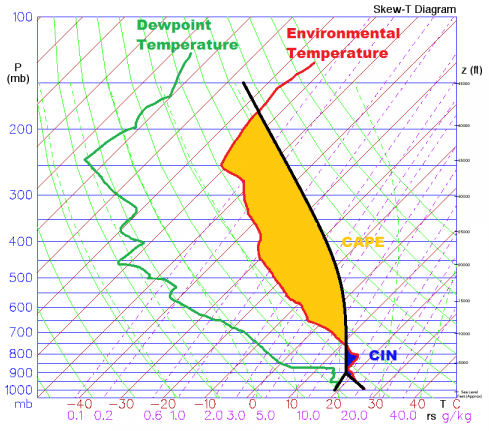
\includegraphics[width=0.35\textwidth]{CAPE.png}
\end{wrapfigure}
    
Las siglas CAPE (Convective Available Potential Energy), hace referencia a la energía potencial disponible para la convección en un momento dado. Es uno de los parámetros que se derivan de los modelos meteorológicos y esta directamente relacionado con el máximo valor potencial de la velocidad vertical de las corrientes ascendentes, por tanto, valores mas altos indican un mayor potencial a clima severo. \\ \\

En tormentas eléctricas, su valor puede exceder los 1000 $J/kg$, y en casos extremos hasta 5000 $J/kg$. CAPE puede ser representado en una gráfica de temperatura contra la presión, siendo su área la encerrada por el nivel de convección libre y el nivel de equilibrio. \\

El Vapor de Agua Precipitable (PW por sus siglas en ingles), indica la cantidad de humedad que hay en un punto fijo. No indica cuanto va a llover, sino mas bien que tanta humedad hay en el aire, además, este valor es también un valor de que tanta humedad hay en el aire por arriba de un lugar. Como se menciono anteriormente, este no indica exactamente que tanto puede precipitar, ya que puede ocurrir la convergencia de la humedad haciendo que la precipitación caiga en un intervalo de tiempo y no instantáneamente. Valores mas altos indican que hay una mayor disponibilidad de humedad para hacer que llueva si la precipitación se va a desarrollar. \\

\begin{wrapfigure}{l}{0.4\textwidth}
    \centering
    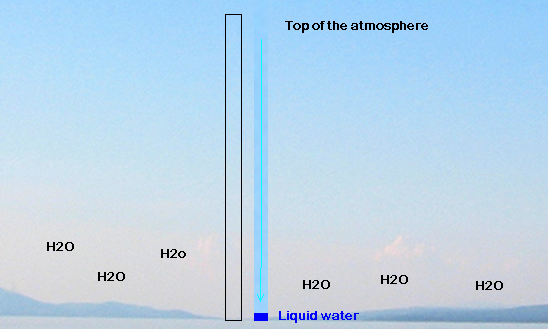
\includegraphics[width=0.4\textwidth]{PW.png}
\end{wrapfigure}
    
Este indicador, tiene implicaciones al prever efectos climatológicos, como lo es la determinación de tormentas severas (la humedad de la troposfera determina si la tormenta tendrá altas precipitaciones, clásicas o bajas) y potencial de inundación (cuando el PW es 2 o 3 veces mas grande que el valor climatológico, es mas probable que ocurra una inundación cuando la precipitación fuerte ocurra). \\

Para nuestro caso, nos interesa la relación entre CAPE y PW, que se puede ver en las tormentas eléctricas: en un valor alto de CAPE, un alto valor de PW, conduce a tormentas que pueden producir demasiados rayos y truenos. 

\section{Limpieza de los archivos}
Para limpiar los archivos primeramente se tomo el archivo creado anteriormente en la practica \#4, en donde se encuentran todos los datos de todos los meses del año de 2017 de la estación del Observador de Valentia. Se realizo un script utilizando el comando egrep, para seleccionar solamente tres renglones en específico, el numero de la estación que contiene la fecha de los lanzamientos, y los dos valores que analizaremos, CAPE y Precipitable Water:

\begin{figure}[h]
    \centering
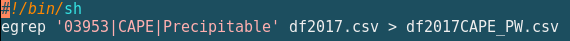
\includegraphics[width=4in]{script1.png}
\end{figure}

Al utilizar este script, se obtuvo el archivo df2017CAPE\_PW.csv, como se muestra a continuación: 

\begin{figure}[h]
    \centering
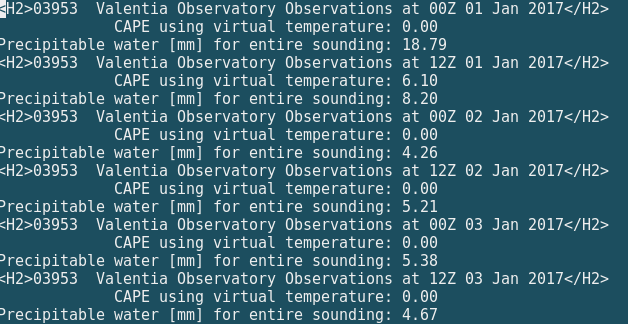
\includegraphics[width=4in]{1archivo.png}
\end{figure}

Para poder utilizar este archivo, tenemos que eliminar todo el texto presente en los datos y juntarlos en un renglón de manera que queden en columnas separados por comas. Esto se hizo con la ayuda del editor de textos emacs, utilizando varias de sus funciones. Primeramente seleccionamos todo el renglón de texto que tiene la estación y su nombre, y paramos hasta antes del lanzamiento, para seleccionarlo se utiliza el comando ctrl + spacebar. Una vez seleccionado, presionamos ctrl + w, para mandar esta linea de texto al "junk", en donde se queda guardado, es un análogo a cortar algo en Word. Si presionamos ctrl+y, se "pega" de regreso lo que "cortamos" anteriormente. Para deshacernos de todos estos renglones (ya que se repiten cada lanzamiento), primero hay que regresarnos al principio del archivo usando el comando ctrl+>. Una vez ahi, presionamos esc+\%, en donde se nos pregunta que es lo que queremos reemplazar, colocamos el texto utilizando ctrl+y, y damos enter. Después de preguntar con que deseamos reemplazarlo, como queremos que no aparezca, lo reemplazamos con nada y para terminar presionamos la tecla !. Esto se hizo con todo el texto que aparece en el archivo. \\

Una vez realizado este proceso, se procedió a juntar los datos en un solo renglón dependiendo del lanzamiento. Esto se hizo de la misma manera que se hablo anteriormente, seleccionando el espacio en blanco y posteriormente eliminándolo usando el comando esc + \%, pero en vez de reemplazarlo con nada, lo reemplazamos con una coma. Por último, se cambiaron los nombres de los meses por su numero correspondiente de la misma manera que colocamos las comas. El archivo quedo de la siguiente manera: 

\begin{figure}[h]
    \centering
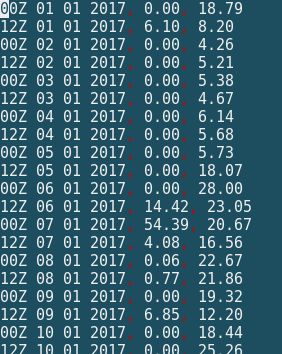
\includegraphics[width=3in]{2archivo.png}
\end{figure}

Ahora, tenemos que dividir los datos dependiendo del lanzamiento que es, 00Z y 12Z. Esto se hizo mediante el uso de un script y el comando egrep, separando los datos en dos lanzamientos, 00Z y 12Z: \\ \\

\begin{figure}[h]
    \centering
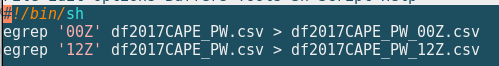
\includegraphics[width=4in]{script2.png}
\end{figure}

Ya que se tienen los archivos separados, eliminamos el texto de 00Z y 12Z, obteniendo nuestro archivo listo para usarse en pandas:

\begin{figure}[h!]
    \centering
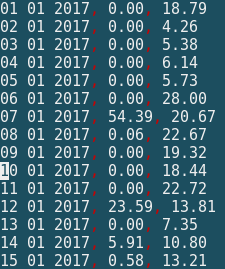
\includegraphics[width=3in]{3archivo.png}
\end{figure}

\section{Análisis de datos}
Con el archivo ya limpio, podemos leerlo utilizando la librería pandas de Python como ya lo hemos hecho anteriormente, excepto que ahora habrá algunas diferencias.  Primero se importaron las mismas librerías que antes, y una nueva, datetime, que se usa para dar formato de fecha a los datos. Ya importadas, colocamos el archivo en un dataframe, indicando que este no tiene cabecera e indicamos sus nombres. Además, el valor de CAPE se transforma a un valor numérico:

\begin{figure}[h!]
    \centering
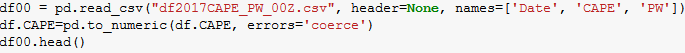
\includegraphics[width=6in]{Ana1.png}
\end{figure}

La columna de fecha también es de tipo objeto, por lo tanto debe transformarse a tipo fecha. Esto se hace con la ayuda de la librería ya mencionada datetime. En este, se indica el formato que tiene la fecha y con esto, el archivo ya esta listo para su análisis: 

\begin{figure}[h!]
    \centering
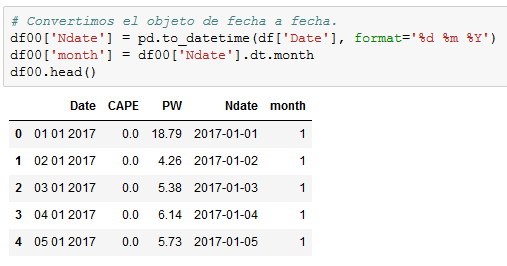
\includegraphics[width=6in]{Ana2.png}
\end{figure}

Para las graficas se utilizaron nuevos tipos de graficas. Estos tipos de graficas permiten ver la relación entre los dos datos, CAPE y PW como parejas para ver si están relacionadas o no, ademas de que una de ellas permite saber que tan sesgados están los datos para saber si su toma es correcta o no. Se utilizo una nueva librería para estas gráficas llamada seaborn, la que nos permite realizar gráficas de caja, gráfica de variables que dependen de ellas o son solamente ellas, y una que muestra la regresión de los datos condicionados a la fecha.

\section{Resultados del análisis}
Primeramente se presenta el diagrama de caja de los dos lanzamientos, para las dos variables distintas:

\begin{figure}[h!]
\begin{subfigure}{.55\textwidth}
  \centering
  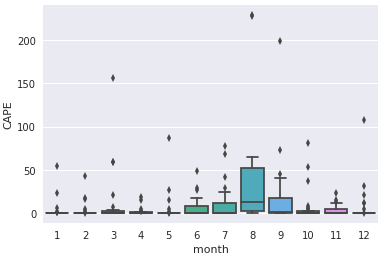
\includegraphics[width=.8\linewidth]{CAPE_mes_00Z.png}
  \caption{Análisis de CAPE}
  \label{fig:sfig1}
\end{subfigure}
\begin{subfigure}{.57\textwidth}
  \centering
  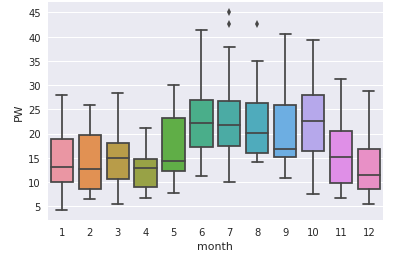
\includegraphics[width=.8\linewidth]{PW_mes_00Z.png}
  \caption{Análisis de PW}
  \label{fig:sfig2}
\end{subfigure}
\caption{Lanzamiento 00Z}
\end{figure}

Como podemos observar en el lanzamiento 00Z, en el caso de CAPE, como la mayoría de las veces este es igual a 0, las medias de los datos están muy cerca de ese valor, y por tanto las cajas tambien. Esto hace que la mayoría de los puntos esten sesgados, es decir, fuera de la caja. La que casi no presenta esto es la del mes de Agosto. En el caso de PW, es casi lo contrario, las cajas están lejanas a 0, y sus puntos no están sesgados (excluyendo en el mes de Junio y Julio). La media de PW en invierno parece estar alrededor de 10 y 20, pero en verano este valor aumenta. 

\begin{figure}[h!]
\begin{subfigure}{.55\textwidth}
  \centering
  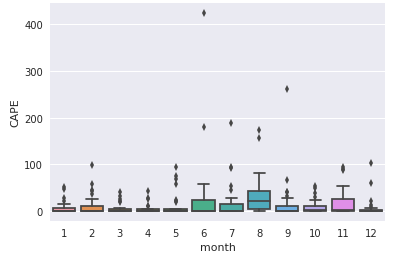
\includegraphics[width=.8\linewidth]{CAPE_mes_12Z.png}
  \caption{Análisis de CAPE}
  \label{fig:sfig1}
\end{subfigure}
\begin{subfigure}{.55\textwidth}
  \centering
  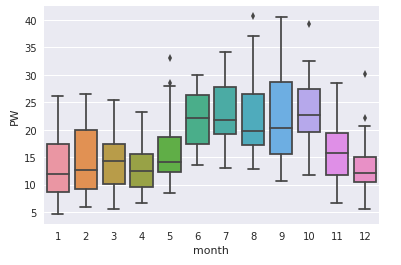
\includegraphics[width=.8\linewidth]{PW_mes_12Z.png}
  \caption{Análisis de PW}
  \label{fig:sfig2}
\end{subfigure}
\caption{Lanzamiento 12Z}
\end{figure}

Para el lanzamiento 12Z, el CAPE al igual que en el lanzamiento anterior, la mayoría de las veces este es igual a 0, las medias de los datos están muy cerca de ese valor, y por tanto las cajas también, pero a diferencia del lanzamiento anterior, este tiene mas puntos sesgados. En el caso de PW, las cajas se alejan aun mas de 0, y tiene mas puntos sesgados que el lanzamiento pasado. Las medias en verano son mayores que las medias que en el lanzamiento 00Z, esto ya que en la tarde la temperatura es mayor. \\

Las graficas en donde se muestra la distribución de los datos como variables separadas y posteriormente como una en función de la otra, para ver si estas se relacionan se presentan a continuación:

\begin{figure}[h!]
\begin{subfigure}{.4\textwidth}
  \centering
  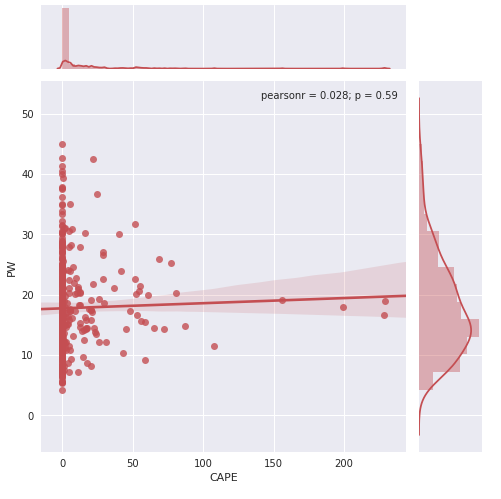
\includegraphics[width=.8\linewidth]{joint_00Z.png}
  \caption{Análisis de 00Z}
  \label{fig:sfig1}
\end{subfigure}
\begin{subfigure}{.4\textwidth}
  \centering
  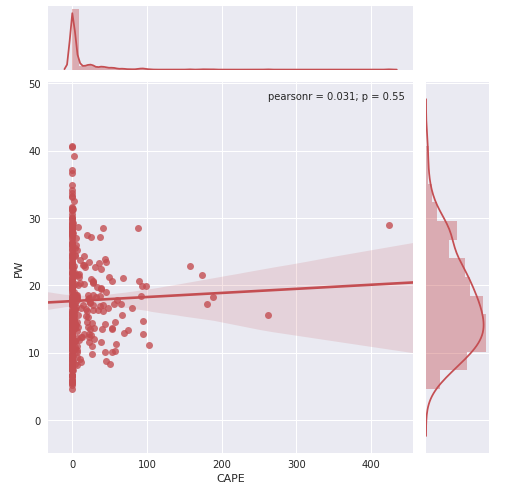
\includegraphics[width=.8\linewidth]{joint_12Z.png}
  \caption{Análisis de 12Z}
  \label{fig:sfig2}
\end{subfigure}
\end{figure}

Como se menciono anteriormente, las graficas de arriba y a la derecha de la gráfica central, muestra la distribución de la variable conforme pasa los días. Siendo la de arriba la correspondiente a CAPE y la lateral a PW. Tanto para 00Z y 12Z son muy parecidas, sin embargo si hay un cambio en la grafica central con la recta que mejor ajusta los puntos para saber si estas están relacionadas o no. El indicador p muestra que no tan relacionados estan los datos, que, como se puede observar son muy altos, a comparación al coeficiente de correlación, por lo cual no se puede observar una relación lineal entre los datos. \\

Por último, se presentan las graficas de la relación de las variables en todo el año:

\begin{figure}[h!]
\begin{subfigure}{.55\textwidth}
  \centering
  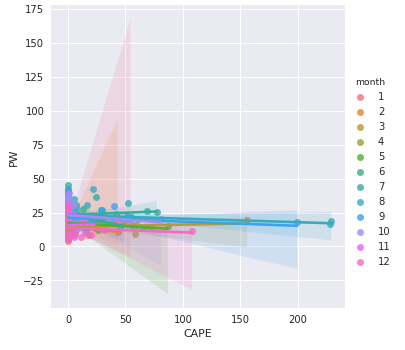
\includegraphics[width=.8\linewidth]{lm_00Z.png}
  \caption{Análisis de 00Z}
  \label{fig:sfig1}
\end{subfigure}
\begin{subfigure}{.55\textwidth}
  \centering
  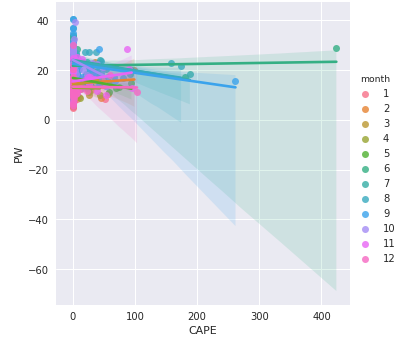
\includegraphics[width=.8\linewidth]{lm_12Z.png}
  \caption{Análisis de 12Z}
  \label{fig:sfig2}
\end{subfigure}
\end{figure}

Como se puede observar para cada mes se forma una recta, y dependiendo de de como cambian las parejas de datos, el triangulo que se forma con la recta cambia de posición. Los triángulos representan la distribución de los datos en cada mes. Como podemos observar, en los lanzamientos 00Z, solamente los triángulos de enero y febrero apuntan hacia arriba, mientras que los demás apuntan hacia abajo. En los lanzamientos de 12Z, todos apuntan hacia abajo. Con esto podemos decir que la relación entre CAPE y PW no es necesariamente lineal. 

\section{Conclusiones}
El análisis de datos no es lo mas difícil para llegar a los resultados que deseamos, es mas bien la limpieza de los datos lo que toma mas tiempo y requiere mas experiencia para facilitar su análisis. Esto ya se había mencionado en reportes anteriores, pero con esta practica solamente queda mas claro que la limpieza de datos es de los procesos mas importantes al analizar datos. Emacs nos permite realizar esto de una manera fácil y ordenada, donde el aprender sus comandos y herramientas permite ser rápido y eficaz al realizar la limpieza de datos. Además, el uso de las nuevas graficas con la librería seaborn, podemos darnos cuenta del poder que tiene python para realizar mas que graficas de variables dependientes, al poder ver graficas de datos estadisticos, y de correlación. 

\section{Bibliografía}
\begin{itemize}
    \item CAPE - Convective Available Potential Energy. (2018) Recuperado de: www.weatheronline.co.uk \\ /reports/wxfacts/CAPE---Convective-Available-Potential-Energy.htm
    \item CAPE y algunas nociones basicas sobre convección atmosferica. (19 de Marzo 2016). www.meteoillesbalears.com/?p=623
    \item What is precipitable water?. Recuperado de: www.theweatherprediction.com/habyhints3/899/
\end{itemize}

Imagenes de:
\begin{itemize}
\item wx4cast.blogspot.mx/2011/10/how-to-read-skew-t-log-p.html
\item http://www.theweatherprediction.com/habyhints3/899/
\end{itemize}

\section{Apéndice}
\noindent\textbf {1. ¿Cómo se te hizo esta actividad? ¿Compleja, Difícil, Sencilla?} \\
Al iniciar la actividad pense que era muy compleja, ya que no tenia mucha experiencia con el uso de emacs, sobre todo en el ámbito de comandos para facilitar la edición. Pero al estudiar y preguntar en clases acerca de los distintos comandos y su uso, la práctica fue mas sencilla de lo que pense. \\

\noindent\textbf {2. ¿Qué te llamó más la atención?}\\
El uso de emacs para la limpieza de datos. En clases anteriores solo lo utilizaba como un editor de textos, pero este tiene muchas mas funciones de las que pensaba. \\

\noindent\textbf {3. ¿Qué parte fue la que menos te interesó hacer? } \\
La verdad no hubo alguna parte de la practica que no me interesara hacer, sin embargo, siento que el hacer un script para solamente una linea de código es algo innecesario. \\

\noindent\textbf {4. ¿Cómo mejorarías esta actividad? ¿Qué le faltó? ¿Qué sobró?} \\
Siento que esta practica estuvo muy completa y el tiempo es suficiente para realizarla. \\

\noindent\textbf {5. ¿Hasta este punto, que te parece el uso de Jupyter para programar en Python?  }\\
Es muy interesante las funciones que tiene panda y matplotlib para el análisis de datos, sobre todo con las nuevas graficas utilizadas, como lo fue la grafica de caja. 
\end{document}